\documentclass[a4paper, fleqn]{article}
\usepackage{enumitem}
\usepackage{amsmath, amssymb}
\usepackage{xstring}
\usepackage{graphicx} % For including figures
\graphicspath{{./figs/}} % Path to figures
% Set engineering notation
\providecommand{\sci}[1]{\protect\ensuremath{\times 10^{\StrSubstitute[0]{#1}{e}{}}}}
\setlength{\parindent}{0pt} % Set paragraph indentation to zero

\begin{document}

\underline{\textbf{Tutorial 3.1: Fastener}}
\vspace{10pt}

% Note - Need direct question.
\textbf{Question 1}
% Unknown kp

\begin{figure}[h]
    \centering
    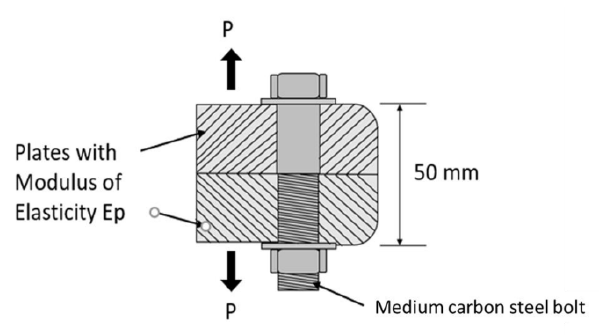
\includegraphics[width=0.5\textwidth]{t31-q1.png}
    \caption{Figure Q1}
\end{figure}

A section of connection illustrated in Figure 1 forms a reusable connection. A total of 4 bolts are used to resist an external load 150 kN. The bolt connection is M14 x 1.5 ISO fine threadclass 5.8, made from medium carbon steel with modulus of elasticity of 200 GPa. The stress in each bolt is 406.2MPa. Determine;

\begin{enumerate}[label=(\roman*)]
    \item The joint stiffness factor.
    \item Stiffness constant for bolt and plates.
    \item Modulus of elasticity of plate Ep
    \item Suggest suitable material used for plates (Based on answer in iii)
\end{enumerate}

\vspace{10pt}
\textbf{Example Solution}
\vspace{10pt}

Reusable connection. Fi = 0.75*Fp\\
No. of bolt $N_{bolt}=4$\\
Load = $150\sci{e+3}N$\\
d=0.014m\\
Pitch, p=1.5mm\\
Fine thread Class 5.8. From table, $S_p=380$MPa\\
$E_b=200\sci{e+9}$Pa\\
$\sigma = 406.2\sci{e6}$Pa\\
From figure, engagement length between parts, L=0.05m
\vspace{10pt}

i-The joint stiffness factor.

\begin{equation} \label{eqjointstiffness}
    \begin{aligned}
    C=\frac{k_b}{k_b+k_p}\\
    \end{aligned}
\end{equation}

$k_b$ and $k_p$ are unknown. Find these two parameter first.

Stiffness constant for bolts, $k_b$
\begin{equation} \label{eqkb}
    \begin{aligned}
    k_b=\frac{A_b \times E_b}{L}
    \end{aligned}
\end{equation}

Cross-sectional area for bolt,

\begin{equation*}
    \begin{aligned}
    A_b &=\frac{\pi d^2}{4}\\
    &= \frac{\pi (0.014)^2}{4}\\
    &= 1.539\sci{e-4}
    \end{aligned}
\end{equation*}

Substitute into Eq. \ref{eqkb},
\begin{equation}
    \begin{aligned}
    k_b &= \frac{1.539\sci{e-4} \times (200\sci{e+9})}{0.05}\\
    &= 6.158\sci{e8}
    \end{aligned}
\end{equation}

$k_p$ cannot be determined because there are unknown values.

Find C from Total force on bolt equation.

Total force on bolt,
\begin{equation} \label{totalForce}
    \begin{aligned}
    F_b=CP+F_i
    \end{aligned}
\end{equation}

Force on the bolt can be found using stress equation.
\begin{equation}
    \begin{aligned}
    \sigma = \frac{F_b}{A}
    \end{aligned}
\end{equation}

\begin{equation*}
    \begin{aligned}
    406.3\sci{e+6} &=\frac{F_b}{\frac{\pi (0.014)^2}{4}}
    \end{aligned}
\end{equation*}

Force on bolt, $F_b=62529.6N$

From Eq.\ref{totalForce}, $F_i$ is still unknown.
Find Preload, $F_i$
\begin{equation*}
    F_i=S_p \times A_t
\end{equation*}
From Table, $S_p=380\sci{e+6}$ and $A_t=125\sci{e-6}$

\begin{equation*}
    \begin{aligned}
    F_i&=380\sci{e+6} \times 125\sci{e-6}\\
    &=35625N 
    \end{aligned}
\end{equation*}

Substitute into Eq.\ref{totalForce}
\begin{equation*}
    \begin{aligned}
    62529 &= C(150\sci{e3})+35625 \\
    C &=0.1793
    \end{aligned}
\end{equation*}

ii - Stiffness constant for bolt and plates.


From Eq.\ref{eqkb}, Stiffness constant for bolt is $k_b=6.158\sci{e8}$

From Eq. \ref{eqjointstiffness}, substitue C and $k_b$ value
\begin{equation*}
    \begin{aligned}
    C &=\frac{k_b}{k_b+k_p}\\
    0.1794 &= \frac{6.158\sci{e8}}{6.158\sci{e8}+k_p} \\
    k_p &=2.817\sci{e9}
    \end{aligned}
\end{equation*}
(No unit)
\vspace{10pt}

iii-Modulus of elasticity of plate Ep

From Eq of $k_p$
\begin{equation}
    \begin{aligned}
        k_p &=\frac{0.58\pi E_p d}{2\ln\left( 5\frac{0.58d+0.5l}{0.58d+2.5l} \right)} \\
        &=2.817\times10^9=\frac{0.58\pi E_p 0.014}{2\ln\left( 5\frac{0.58(0.014)+0.5(0.05)}{0.58(0.014)+2.5(0.05)} \right)}\\
        &=2.284\sci{e11}\\
        &=228.4GPa
    \end{aligned}
\end{equation}


iv - Suggest suitable material used for plates (Based on answer in iii)


\end{document}